% !TEX program = xelatex
\documentclass[12pt,a4paper]{ctexart}

% ===== Packages =====
\usepackage{geometry}
\geometry{left=2.5cm,right=2.5cm,top=2.5cm,bottom=2.5cm}

\usepackage{graphicx}
\graphicspath{{report_figures/}}
\usepackage{subcaption}
\usepackage{hyperref}
\usepackage{enumitem}
\usepackage{booktabs}
\usepackage{listings}
\usepackage{xcolor}
\usepackage{tikz}
\usetikzlibrary{positioning}
\usepackage{float}
\usepackage{multirow}

% Code listing style
\lstset{
  basicstyle=\ttfamily\small,
  breaklines=true,
  frame=single,
  numbers=none,
  language=Python,
  keywordstyle=\color{blue},
  commentstyle=\color{gray},
}

\hypersetup{
  colorlinks=true,
  linkcolor=blue,
  urlcolor=blue,
}

\setlength{\parskip}{0.5em}
\setlength{\parindent}{2em}

% ===== Title =====
\title{MathSolver：基于LLM的微积分与概率论\\智能解题与批改系统}
\author{项目报告}
\date{\today}

\begin{document}

\maketitle

\begin{abstract}
\noindent MathSolver是一个面向微积分与概率论领域的LLM智能体系统，遵循ToRA与SelfCheck范式，结合符号计算引擎SymPy/scipy、MCP外部工具调用，实现了数学问题的自动求解与逐步批改。系统采用19类问题模式（Schema）驱动的提示工程，支持单路径推理与USC多路径自洽性采样，并在批改阶段引入PARC前提链验证与元验证机制以降低误判风险。本文从系统架构、核心模块和评测体系等方面对该项目进行说明。

关键词：LLM智能体；数学求解；SymPy；MCP；USC自洽性；Gradio
\end{abstract}

% ======================================================================
\section{问题背景与动机}
% ======================================================================

在辅导同学微积分的过程中，笔者观察到一个普遍现象：不少同学拿到标准答案后能“看懂”答案的每一步推导，却依然无法判断自己原本的解答到底错在哪一步、为什么错。标准答案只展示“正确路径”，而学生真正需要的是对自己思维过程的逐步诊断——告诉他们哪一步前提缺失、哪一步推理跳跃、哪一步计算错误，并给出修正方向。传统作业批改受限于教师精力，往往只能给出对错判定或简短评语；通用大语言模型虽然能讲解答案，却难以稳定地“对照学生自己的步骤”做出细粒度反馈，也容易在不验证的情况下产生幻觉式批改。

MathSolver 正是为弥补这一缺口而构建的智能体：它以学生手写解答为输入，自动识别步骤、对照标准解法进行逐步批改，并给出每一步的置信度与正误判断，辅以元验证机制防止批改本身的误判。系统还提供“举一反三”功能，帮助学生针对自己暴露的薄弱点进行针对性练习。通过将 LLM 推理与符号计算工具（SymPy、SciPy）结合，项目力图让“个性化步骤诊断”在工程上可靠落地。

% ======================================================================
\section{项目概述}
% ======================================================================

MathSolver是一个基于大语言模型（LLM）的数学问题求解与批改系统，聚焦微积分与概率论两个领域。项目将LLM的推理能力与符号计算工具（SymPy、SciPy）相结合，使LLM负责规划推理路径并生成代码，工具侧负责执行与验证，从而实现数学问题的端到端求解以及学生解答的自动化批改。

该系统采用Python 3.10+开发，以Gradio 6+作为前端框架，通过OpenAI兼容API调用LLM模型，并利用MCP（Model Context Protocol）整合外部数学工具。系统完整源代码托管于GitHub：\url{https://github.com/THUapm/cal_solver}。

\subsection{核心特性}

\begin{itemize}[nosep]
  \item 智能求解：支持19种微积分与概率论问题模式，涵盖积分、导数、极限、概率分布、贝叶斯推断、最大似然估计、假设检验、置信区间等。
  \item 逐步批改：基于PARC前提链验证的5类错误分类体系，辅以元验证机制防止误判。
  \item USC自洽性：对高难度问题启用多路径采样（N=3），并采用2/3早退策略，在节省约33\%计算开销的同时保持答案可靠性。
  \item 验证—修正闭环：求解后自动进行自我验证；检测到错误时进入定向修正循环，最多执行2轮。
  \item 5项MCP工具：覆盖符号计算、数值概率、结果验证、函数绘图与LaTeX语法校验。
\end{itemize}

% ======================================================================
\section{系统架构}
% ======================================================================

MathSolver的整体架构可以概括为"前端展示—核心编排—工具执行"三个层次。

\begin{figure}[H]
\centering
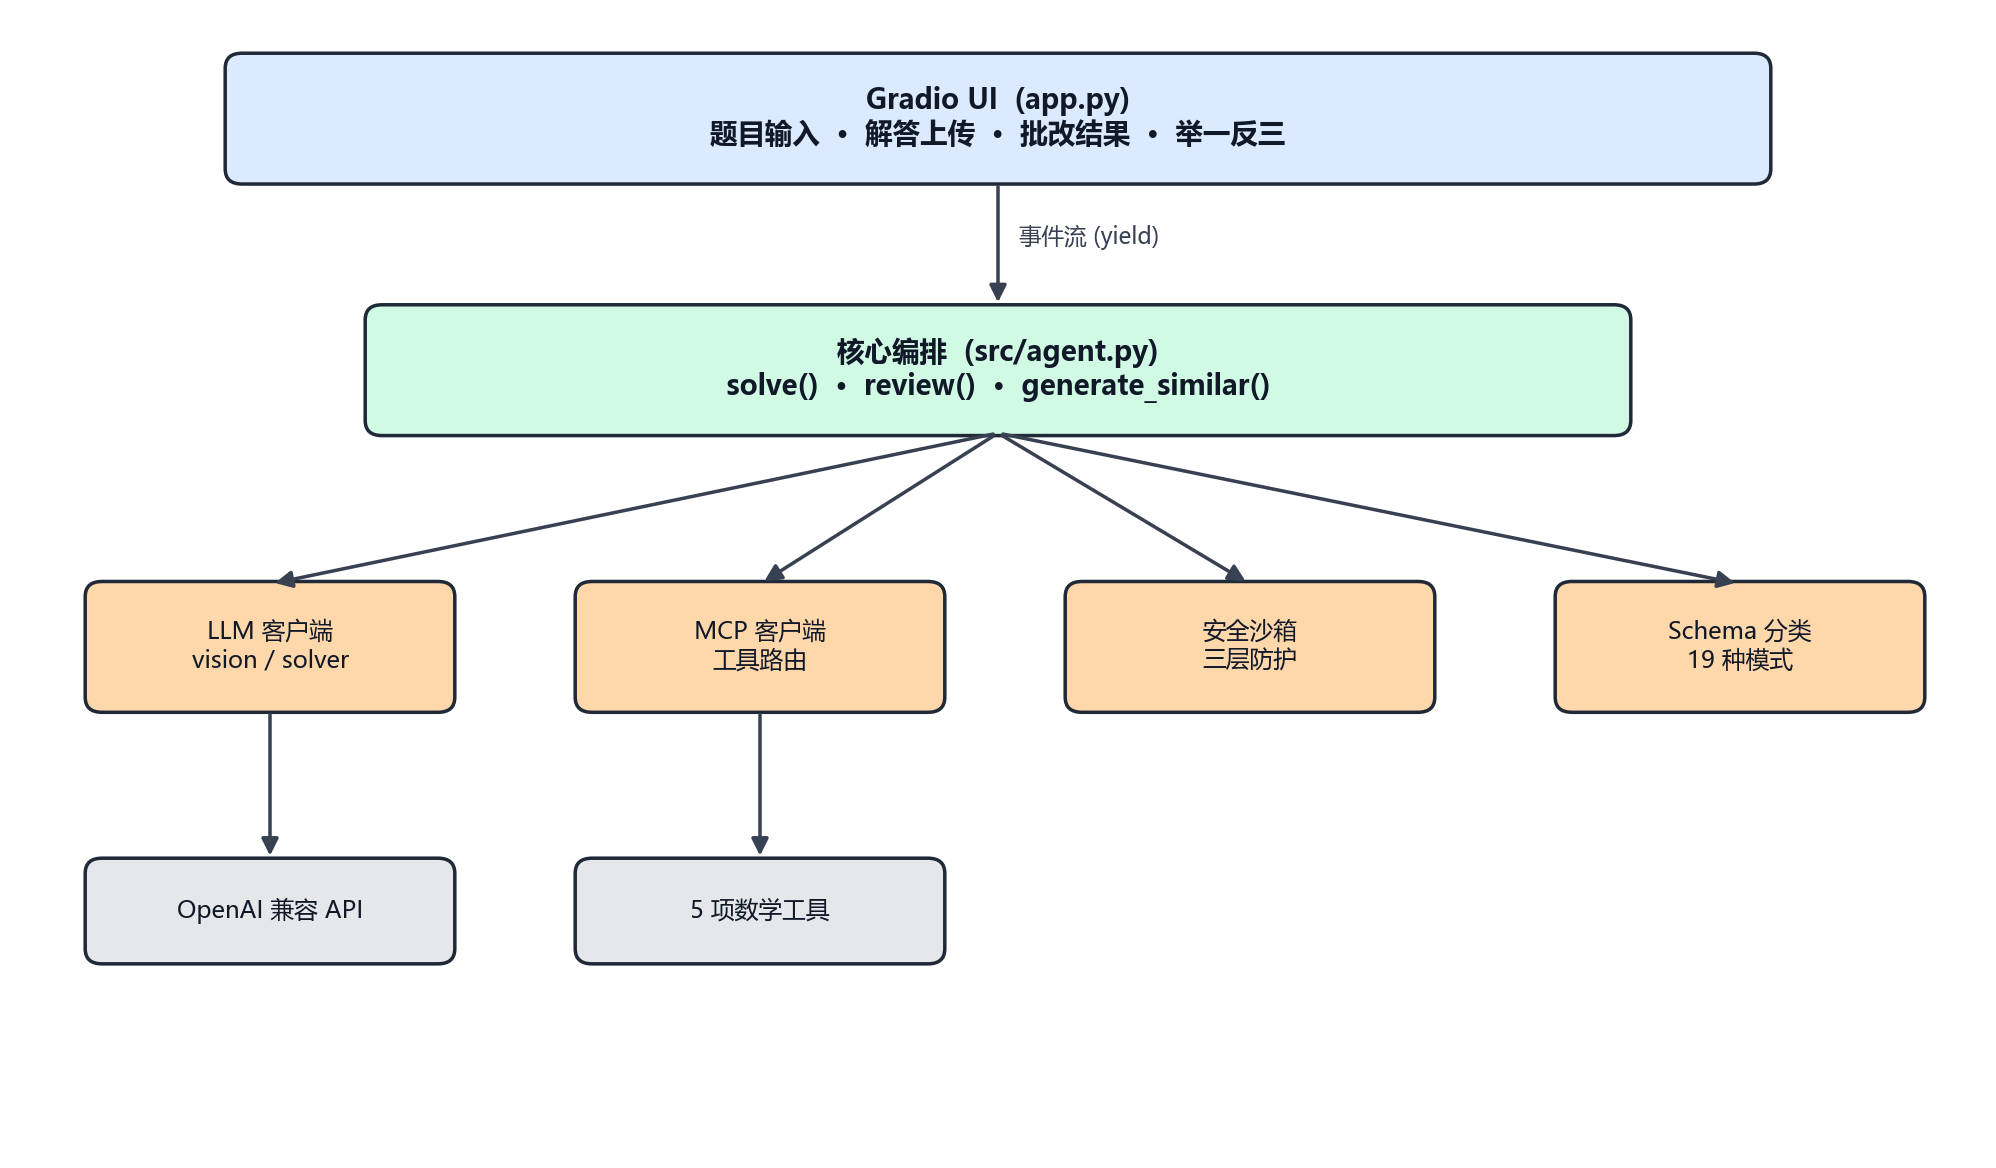
\includegraphics[width=0.95\textwidth]{architecture.png}
\caption{MathSolver 系统架构}
\label{fig:arch}
\end{figure}

\subsection{事件驱动的Generator模式}

系统的核心函数\texttt{solve()}、\texttt{review()} 和 \texttt{generate\_similar\_problems()} 均采用 Python Generator 模式实现。每个函数运行过程中通过 \texttt{yield} 向外发送事件字典，例如 \texttt{step\_start}、\texttt{step\_done}、\texttt{final} 等事件类型，前端 Gradio UI 迭代消费这些事件，从而展示实时进度。

该设计的优点包括：无需注册回调函数，代码流程清晰；前端可随时呈现推理的中间状态；生成器支持嵌套——\texttt{solve\_multi\_path()} 内部调用 \texttt{solve\_single\_path()}，事件透传路径明确。

% ======================================================================
\section{智能求解模块}
% ======================================================================

\subsection{问题模式分类}

系统设计了19种数学问题的模式（Schema），覆盖微积分（12种）和概率与统计推断（7种）两大领域。模式分类采用关键词匹配策略：每个Schema包含一组关键词（含中英文），通过计算问题文本与各模式关键词的交集得分，选择最高分模式作为问题类型。

\begin{table}[H]
\centering
\caption{问题模式分类概览}
\begin{tabular}{@{}lll@{}}
\toprule
\textbf{领域} & \textbf{模式} & \textbf{示例关键词} \\
\midrule
\multirow{4}{*}{微积分} & 换元积分、分部积分、定积分、三角积分 & 换元、$u$-substitution、$\int$\\
                        & 极限计算、洛必达法则 & limit、$\to 0$、$0/0$型\\
                        & 导数、高阶导数、偏导数 & derivative、$f'(x)$、$\partial f$\\
                        & 泰勒展开、方程求解、优化极值 & Taylor、solve、极值\\
\midrule
\multirow{4}{*}{概率统计} & 贝叶斯定理、二项/正态/泊松分布 & Bayes、Binomial、$N(\mu,\sigma)$\\
                        & 组合计数、条件概率 & $C(n,k)$、$P(A\mid B)$\\
                        & 期望方差、连续分布 & $E[X]$、CDF、PDF\\
                        & MLE、充分统计量、假设检验 & 最大似然、$H_0$、p-value\\
                        & 置信区间、贝叶斯推断 & $1-\alpha$、先验、后验\\
\bottomrule
\end{tabular}
\end{table}

每个模式包含步骤模板（英文，直接注入LLM提示）、常见陷阱和验证策略。模式信息通过\verb|build_schema_injection()|嵌入系统提示，引导LLM按领域最佳实践组织推理。

\subsection{单路径求解流程}

\verb|solve_single_path()|实现核心的推理-执行-验证循环：

\begin{enumerate}[nosep]
  \item 提示构建：将系统提示、模式注入、MCP工具描述、10道few-shot示例以及安全防护指令组装为完整的系统消息。
  \item 迭代推理（最多5轮）：
    \begin{itemize}[nosep]
      \item LLM生成推理文本，其中包含Python代码块（以 \texttt{python} 标记）和/或MCP工具调用块（以 \texttt{tool} 标记）
      \item 系统解析并执行代码（通过安全沙箱），调用MCP工具获取外部计算结果
      \item 执行结果以工具消息形式反馈给LLM，继续下一轮推理
    \end{itemize}
  \item 最终答案检测：通过正则匹配\verb|\boxed{}|、\verb|最终答案|等模式判断LLM是否已得出结论。
  \item 验证阶段：LLM对自身解答进行自检，发现错误时进入修正循环（最多2次）。
\end{enumerate}

\subsection{多路径自洽性（USC）}

对于被判定为\texttt{hard}难度的问题，系统采用Universal Self-Consistency（USC）策略。\verb|solve_multi_path()|使用不同温度参数（0.3、0.45、0.6）生成3条独立推理路径。

B1早退机制：运行完前2条路径后，比较提取的最终答案。若一致，立即终止第3条路径并返回结果，节省约33\%的token消耗。若3条路径的答案各不一致，则将全部解答提交给LLM选择最优路径。答案一致性检测支持数值浮点比较（相对容差0.1\%）和字符串标准化比较。

\subsection{验证优先自动修正}

系统在单路径求解完成后，自动进入验证优先（Verify-First）阶段：

\begin{enumerate}[nosep]
  \item 向LLM发送验证提示（\verb|VERIFICATION_PROMPT|），要求其逐项检查逻辑正确性、计算准确性、边界条件
  \item 解析验证响应中的错误标记——先检查显式否定语句（如"no error"等），再检查直接错误符号（如×），最后匹配间接错误关键词（如"incorrect"、"计算错误"等）
  \item 若检测到错误，生成针对性修正提示（\verb|build_correction_prompt()|），仅要求修正错误步骤而非重新解答
  \item 修正后再次验证，最多2轮循环
\end{enumerate}

% ======================================================================
\section{智能批改模块}
% ======================================================================

\subsection{PARC前提链验证}

批改模块的一个重要设计是前提链验证（Premise-chain Verification）。系统首先调用\verb|solve()|生成标准参考解，随后对学生解答的每一步提取其逻辑前提：

\begin{itemize}[nosep]
  \item \textbf{Step 0}：原始问题陈述，是所有步骤的基础前提
  \item Step N的前提：LLM分析当前步骤直接依赖的先前步骤编号，输出为JSON格式的前提图（DAG）
  \item 前提提取提示（\verb|PREMISE_EXTRACTOR_PROMPT|）强调"宁可多包含前提，不可遗漏"
\end{itemize}

前提链以有向无环图（DAG）的形式组织，使得后续错误分析可以区分原生错误（该步骤自身出错）与累积错误（继承自错误前提）。

\subsection{五类错误分类}

批改系统定义了5种错误类别：

\begin{table}[H]
\centering
\caption{错误分类体系}
\begin{tabular}{@{}lp{9cm}@{}}
\toprule
\textbf{类别} & \textbf{描述} \\
\midrule
CALCULATION\_ERROR & 计算/代数运算错误（算错数字、符号错误、抄写错误） \\
LOGIC\_ERROR & 推理无效、等价关系错误、无依据的假设 \\
CONCEPT\_ERROR & 定理/公式误用、概念理解错误 \\
NOTATION\_ERROR & 符号/括号错误、单位错误 \\
ACCUMULATION\_ERROR & 步骤自身逻辑正确，但因依赖错误前提而传递错误 \\
\bottomrule
\end{tabular}
\end{table}

每次批改首先识别原生错误（原生错误检测独立于前提），然后通过DAG检测累积错误：若某步骤的所有前提均正确，但该步骤依赖了某个已被标记为错误的先前步骤，则自动标记为\verb|ACCUMULATION_ERROR|并追溯根因。

\subsection{元验证：防止误判}

为防止LLM将学生的正确步骤误判为错误（即产生"幻觉"），批改完成后进入元验证（Meta-Check）阶段：

\begin{itemize}[nosep]
  \item 将问题、学生解答、批改结果一同提交给LLM，要求逐项审查每个×标记是否为真实错误
  \item 输出格式为\verb|CONFIRMED|（确认错误存在）或\verb|REJECTED|（批改判断有误，该步骤实际正确）
  \item 若任何判断被\verb|REJECTED|，提供修正后的批改结果
\end{itemize}

元验证的触发条件与问题难度挂钩：简单题不触发，中等题仅在检测到错误时触发，难题始终触发。

% ======================================================================
\section{MCP工具系统}
% ======================================================================

系统通过MCP协议整合了5项外部数学工具，运行于独立进程，通过标准输入输出（stdio）与主程序通信：

\begin{table}[H]
\centering
\caption{MCP工具一览}
\begin{tabular}{@{}llp{7cm}@{}}
\toprule
\textbf{工具} & \textbf{功能} & \textbf{典型调用} \\
\midrule
symbolic\_compute & SymPy符号计算 & 微分、积分、极限、解方程、化简 \\
numerical\_probability & scipy.stats分布计算 & CDF/PDF/PMF、分位数、期望、方差 \\
verify\_result & 交叉验证 & 求导验证积分、多点数值代入验证、边界检查 \\
plot\_function & 函数绘图 & 生成PNG图像（base64编码） \\
latex\_validate & LaTeX语法校验 & 括号匹配、表达式解析 \\
\bottomrule
\end{tabular}
\end{table}

MCP工具的调用由LLM自主决策：在提示中显式区分\texttt{python}代码块（对应本地沙箱执行）与\texttt{tool}代码块（对应MCP远程调用），LLM根据任务需要选择合适的方式。工具描述通过\texttt{format\_mcp\_tools\_for\_prompt()}自动从MCP服务器的inputSchema生成结构化文档注入系统提示。

% ======================================================================
\section{提示工程}
% ======================================================================

\subsection{分层提示架构}

系统的提示体系由以下层次组成：

\begin{itemize}[nosep]
  \item 基础层：求解系统提示词，定义 LLM 的角色、工作流程和输出格式要求
  \item 策略增强层：验证优先策略 + 主动交叉验证指令
  \item 领域注入层：Schema 模式信息 + 微积分 / 概率论参考知识
  \item 工具层：MCP 工具描述
  \item 示例层：10 道概率论与统计推断 few-shot 示例（约 450 行），覆盖 8 种分布模式与 5 种推断模式
  \item 安全层：不可信内容包裹与注入防护指令
\end{itemize}

总计，每次求解的系统提示约5000—8000 token（含10道完整示例）。输出格式要求包含5个标准段落（问题分析、解题方法、逐步计算、结果验证、最终答案），每个计算步骤须附验证代码。

\subsection{输出规范}

提示中明确要求LLM不得在回复中夹杂内部元叙述（如"输出："、"我们还可以"、"Step N:"等），以免将代理间通信信息暴露给终端用户。\verb|strip_code_blocks()|在后处理阶段进一步清除LLM输出中的元信息、重复编号以及中文重复片段。

% ======================================================================
\section{评测体系}
% ======================================================================

\subsection{评估指标}

系统在\verb|eval/metrics.py|中实现了4项核心评测指标：

\begin{itemize}[nosep]
  \item 步骤准确率（Step Accuracy）：精确率/召回率/F1/准确率，评估LLM判定步骤正确与否的二分类性能
  \item 期望校准误差（ECE）：将置信度（0—100）分10档，比较每档的平均预测置信度与实际正确率的差距
  \item \textbf{Brier Score}：概率预测质量指标，范围[0,1]，越小越好
  \item \textbf{Cohen's Kappa}：分类一致性指标，衡量预测错误类别与真实错误类别的一致性
\end{itemize}

同时还计算辅助指标：低置信度步骤（$<$70）中的实际正确率和 高置信度步骤（$\geq$90）中的实际正确率，用于检测LLM的过度自信或自信不足。

\subsection{评测数据集}

项目提供两个评测入口：

\begin{itemize}[nosep]
  \item PRM800K评测（\verb|eval/run_prm800k_eval.py|）：基于OpenAI PRM800K数据集的步骤级正误标签评测。PRM800K包含80万条步骤级标注，评测集500题。
  \item 图片解答评测（\verb|eval/run_pic_eval.py|）：对手写图片解答进行端到端批改评测，含ground truth步骤正误标签。
\end{itemize}

% ======================================================================
\section{用户界面}
% ======================================================================

前端采用Gradio 6+框架，使用自定义Linear-style主题（\verb|assets/theme.py|定义LinearLight色板），搭配自定义CSS（\verb|assets/style.css|）和HTML头部（Inter + JetBrains Mono字体、主题切换）。页面采用单列四步流程，避免复杂多栏布局对移动端和截图展示造成干扰。

UI分为四个模块：

\begin{enumerate}[nosep]
  \item 题目输入：支持文字输入和图片上传，提供6道内置示例
  \item 解答上传：支持手写/电子解答图片OCR识别
  \item 批改结果：逐步批改展示，每步附颜色徽章（绿色$\geq$90\%置信度+正确、黄色70—89\%、红色$<$70\%或错误）+ 元验证结果
  \item 举一反三：按钮始终可见（批改前禁用、批改后启用），根据题目知识点自动生成3道同类型练习题
\end{enumerate}

公式渲染从客户端 KaTeX 迁移为服务端 MathML：Gradio 6.x 模板不再可靠注入 \texttt{head=} 内容，因此项目在 Python 端用 \texttt{latex2mathml} 把 LaTeX 转换为 MathML，再写入 \texttt{gr.HTML}。

\texttt{latex\_to\_html()} 采用两阶段管道：

\begin{enumerate}[nosep]
  \item 先将四种公式分隔符（\texttt{\$\$...\$\$}、\texttt{\textbackslash[...\textbackslash]}、\texttt{\textbackslash(...\textbackslash)}、\texttt{\$...\$}）转换并暂存为自定义 HTML 元素 \texttt{<mslot data-i="N">} 占位符；
  \item 按空行进行 block-aware Markdown 转换，生成结构化 HTML（标题、列表、段落分别用对应标签）；
  \item 最后恢复 MathML，把占位符替换为公式渲染结果。
\end{enumerate}

占位符选型经过三次迭代：早期 \texttt{\textbackslash x00MATH} 的 null 字节在 JSON 序列化中被吞；中期的 \texttt{@@MATH@@} 与 LLM 输出字面冲突；最终选用 \texttt{<mslot>} 自定义元素，能稳定通过 Gradio sanitizer 且不会与文本内容冲突。

\begin{figure}[H]
\centering
\begin{minipage}{0.46\textwidth}
\centering
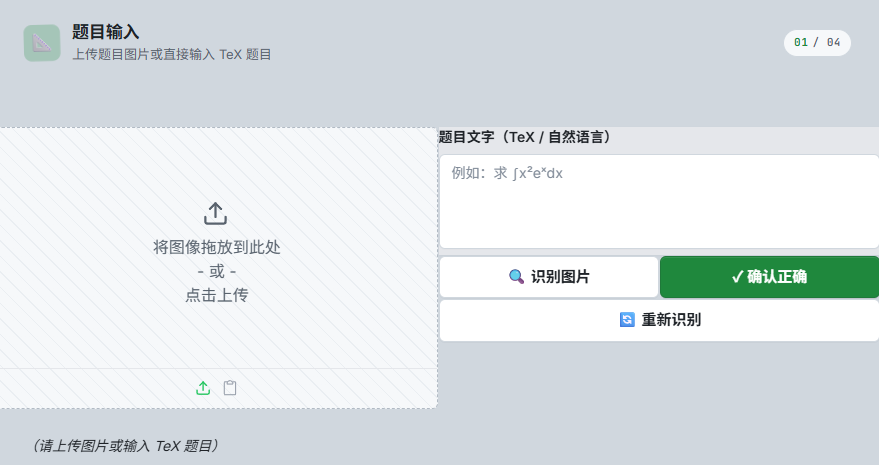
\includegraphics[width=\textwidth]{01_upload.png}
\subcaption{题目输入与示例选择}
\end{minipage}\hfill
\begin{minipage}{0.46\textwidth}
\centering
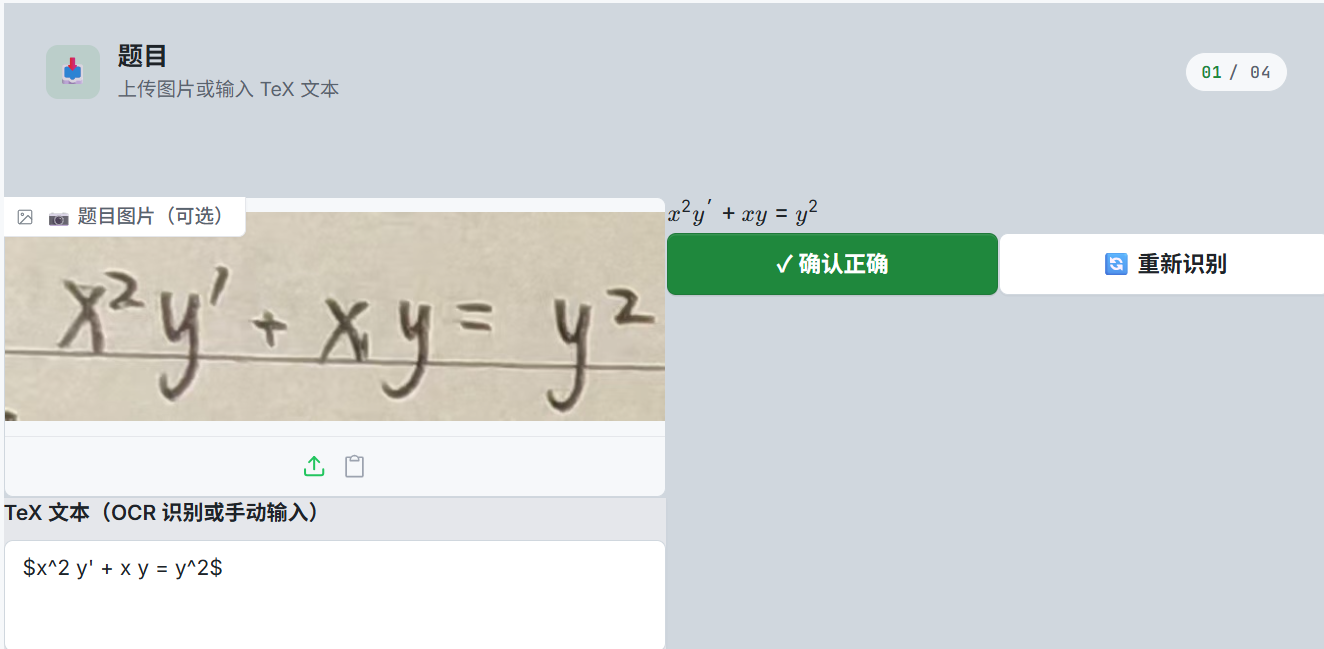
\includegraphics[width=\textwidth]{02_ocr_preview.png}
\subcaption{OCR识别+MathML公式渲染}
\end{minipage}

\vspace{0.5em}

\begin{minipage}{0.46\textwidth}
\centering
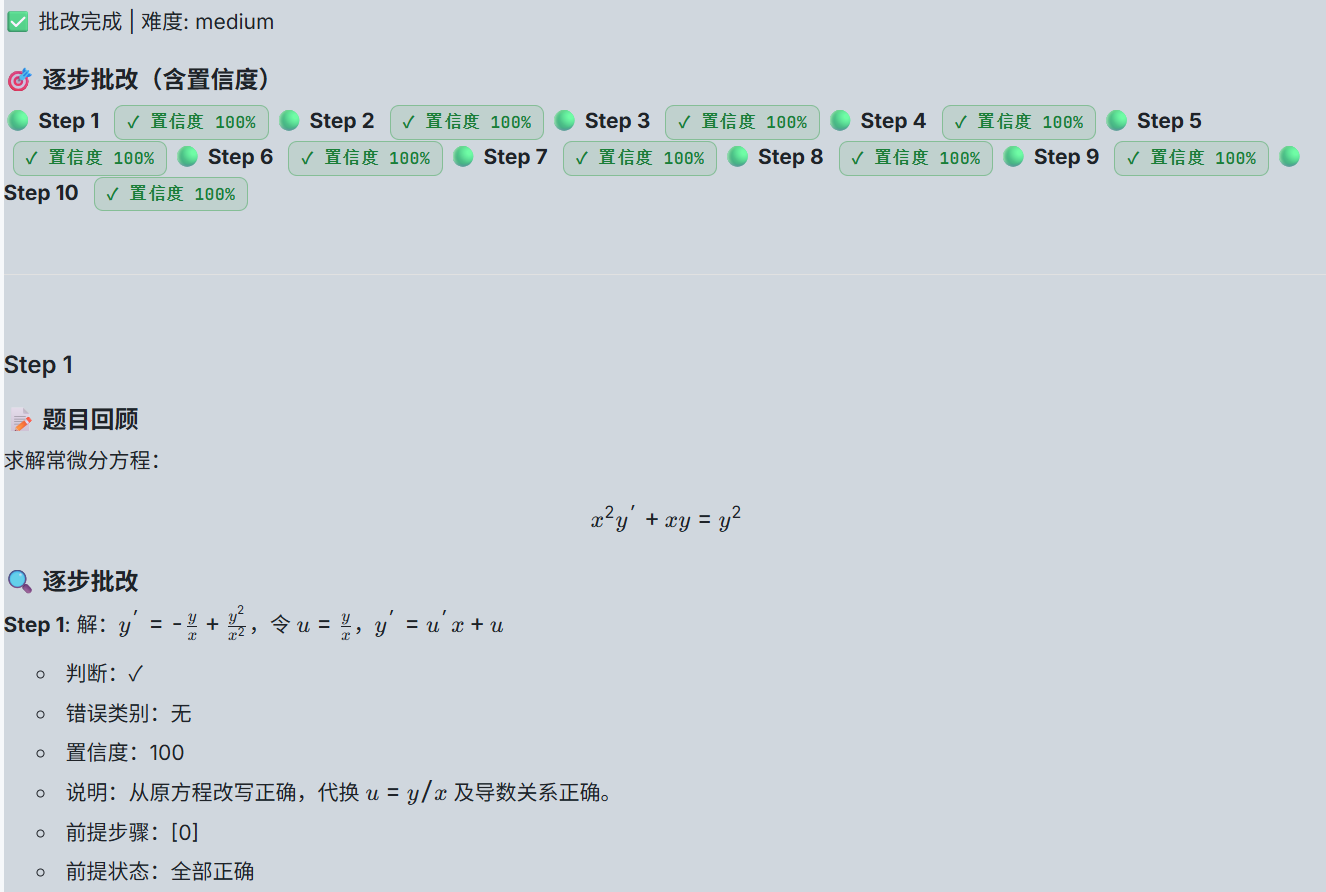
\includegraphics[width=\textwidth]{03_grading_result.png}
\subcaption{逐步批改+置信度徽章+元验证}
\end{minipage}\hfill
\begin{minipage}{0.46\textwidth}
\centering
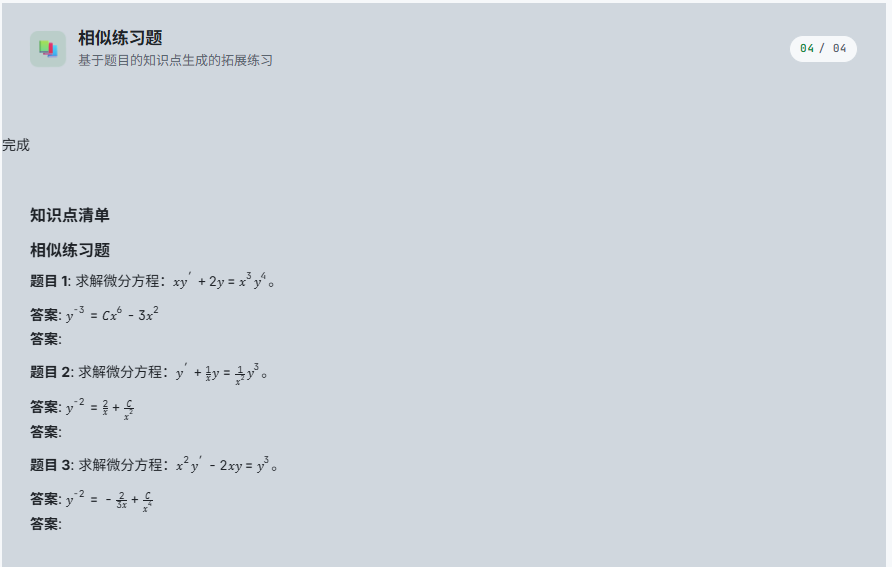
\includegraphics[width=\textwidth]{04_similar_problems.png}
\subcaption{举一反三+相似题生成}
\end{minipage}
\caption{前端四大核心场景截图}
\label{fig:ui}
\end{figure}

% ======================================================================
\section{部署与运行}
% ======================================================================

\subsection{环境配置}

\begin{itemize}[nosep]
  \item Python 3.10+，依赖包括 SymPy $\geq$1.12、SciPy $\geq$1.11、OpenAI $\geq$1.0、Gradio $\geq$6.0、MCP $\geq$1.2.0、Matplotlib $\geq$3.7、latex2mathml
  \item 环境变量通过 \texttt{.env} 文件配置（模板：\texttt{.env.example}），必须项为 \texttt{API\_KEY}
  \item MCP 工具通过 \texttt{config/mcp\_servers.json} 配置（模板同目录下的 \texttt{.example} 后缀文件），两项配置文件均被 \texttt{.gitignore} 排除
\end{itemize}

\subsection{运行方式}

启动流程为三步：（1）用 \texttt{pip} 安装依赖；（2）复制 \texttt{.env.example} 为 \texttt{.env} 并填入 \texttt{API\_KEY}；（3）运行 \texttt{python app.py} 启动 Gradio，浏览器访问 \texttt{localhost:7860} 即可。

\subsection{测试运行}

项目无标准测试框架，使用4个独立的\verb|assert|式测试脚本：\verb|test_p0_fixes.py|（安全沙箱+LLM客户端+注入防护，32项）、\verb|test_skills.py|（模式分类+USC+few-shot，14项）、\verb|test_examples.py|（代码执行器+解析器+B1/B2生成器，11项）、\verb|test_mcp.py|（MCP工具解析，离线/在线8项）。所有离线测试无需API Key即可通过。

% ======================================================================
\section{工作量说明}
% ======================================================================

依据课程要求，此处如实说明各项工作来源，以便评判工作量：

\begin{itemize}[nosep]
  \item 本人完成：
  \begin{itemize}[nosep]
    \item 工作流设计与架构决策（USC 早退、PARC 前提链、Verify-First 闭环、元验证、三层沙箱防御、5 类错误分类体系）；
    \item 查找与研读 13 篇相关论文（PRM800K、过程奖励模型、置信度校准等方向）；
    \item 本报告撰写。
  \end{itemize}
  \item 大模型完成：大部分代码实现与提示工程交由 Claude Code / GLM 在本人给出明确需求与设计后生成，本人审阅并调试。涉及模块包括 \texttt{src/agent.py} 核心 Generator 事件流、\texttt{src/utils.py} 解析与渲染逻辑、\texttt{safe\_runner.py} 安全沙箱、\texttt{app.py} Gradio 前端、\texttt{assets/} 主题与 CSS、4 套测试脚本、\texttt{src/prompts.py} 分层提示与 few-shot 示例。
  \item 第三方资源：SymPy / SciPy / OpenAI Python SDK / Gradio / MCP / Matplotlib / latex2mathml 等开源库；数学题素材取自公开教材与课堂例题。
\end{itemize}

% ======================================================================
\section{总结与展望}
% ======================================================================

\subsection{技术亮点}

\begin{enumerate}[nosep]
  \item 模式驱动提示：19种问题模式为LLM提供了领域知识锚点，使得推理过程的结构化程度明显提高。
  \item USC多路径推理：N=3路径采样配合B1早退策略，在答案准确性与计算开销之间取得了平衡。
  \item 验证优先—自动修正闭环：求解后立即启动自检，发现问题后进入最多2轮定向修正，构成自我改进循环。
  \item PARC前提链批改：基于DAG的前提链验证将错误区分为原生错误与累积错误，结合元验证有效降低了误判率。
\end{enumerate}

\subsection{局限与改进方向}

\begin{enumerate}[nosep]
  \item 模式分类精度：当前采用简单关键词匹配，对于表述模糊的问题可能匹配到错误模式。未来可考虑使用LLM进行更精准的few-shot分类。
  \item 评测数据规模：PRM800K评测集仅选用500题的小规模子集，图片评测用例也较为有限（2个）。扩大评测规模可提供更可靠的性能指标。
  \item 错误分类一致性：五类错误的定义在不同LLM之间可能存在差异，需要更严格的一致性评估。
  \item 多模态支持：当前OCR依赖独立的Vision模型调用，未实现端到端的多模态推理。
  \item 实时性能：USC多路径推理和元验证环节引入了额外延迟，对于简单题目存在不必要的计算开销。
\end{enumerate}

\subsection{未来工作}

后续工作可沿以下几个方向推进：增加线性代数、微分方程等新的数学领域模式；引入检索增强生成（RAG）知识库，纳入教材和定理资源；实现更细粒度的前提链验证，不仅识别步骤间的依赖关系，也评估前提被使用的正确性；以及开发浏览器扩展或移动端接口，降低师生的使用门槛。

\vspace{1cm}
\noindent 项目地址：\url{https://github.com/THUapm/cal_solver}

\noindent 许可证：MIT License

\end{document}
